\documentclass[12pt]{ociamthesis}  % default square logo 
%\documentclass[12pt,beltcrest]{ociamthesis} % use old belt crest logo
%\documentclass[12pt,shieldcrest]{ociamthesis} % use older shield crest logo

%load any additional packages
\usepackage{amssymb}
\usepackage{multirow}
\usepackage{caption}
\usepackage{titlesec}
\usepackage{charter}
\usepackage{subfiles}
\usepackage{etoolbox} %halaman I-1
%\patchcmd{\addcontentsline}
 % {\thepage}
  %{\thechapter-\thepage}
  %{}
  %{}

\makeatletter
\@addtoreset{subsubsection}{chapter}
\makeatother
\renewcommand{\thepage}{\thechapter-\number\numexpr\arabic{page}\relax}
\patchcmd{\cleardoublepage}{\ifodd}{\unless\ifodd}{}{}
\preto\chapter{\cleardoublepage}
\AtBeginDocument{\setcounter{page}{1}}





\makeatletter					%
\renewcommand*\@pnumwidth{3em}	% ratain halaman daftar isi
\makeatother					%

\title{\large RESUME PYTHON\\[1ex]     %your thesis title,
        }   %note \\[1ex] is a line break in the title
        

\author{Diajukan untuk memenuhi kelulusan matakuliah Pemrograman II 
pada Program Studi DIV Teknik Informatika\\[5ex]
O l e h : \\
[1ex] Siti Nurhayati Puja Kesuma   \\ 
\textbf{1.18.4.004}\\
		 [5ex] } 
		 
\college{}  %your college

%\renewcommand{\submitt edtext}{change the default text here if needed}
\degree{POLITEKNIK POS INDONESIA}    %the degree
\degreedate{\textbf{BANDUNG\\2019}}  

%end the preamble and start the document
\begin{document}

%this baselineskip gives sufficient line spacing for an examiner to easily
%markup the thesis with comments
\baselineskip=18pt plus1pt

%set the number of sectioning levels that get number and appear in the contents
\setcounter{secnumdepth}{3}
\setcounter{tocdepth}{3}


\maketitle          % create a title page from the preamble info

   
\chapter{Mengenal Python dan Anaconda}
Tujuan pembelajaran pada pertemuan pertama antara lain:
\begin{enumerate}
\item
Mengerti sejarah python, perkembangan dan penggunaan python di perusahaan
\item
Memahami tahapan instalasi python dan anaconda
\item
Memahami cara penggunaan spyder
\end{enumerate}
Tugas dengan cara dikumpulkan dengan pull request ke github dengan menggunakan format latex pada repo yang dibuat oleh asisten IRC.

\section{Teori}
Praktek teori penunjang yang dikerjakan :
\begin{enumerate}
\item
Buat Resume Sejarah Python, perbedaan python 2 dan 3, dengan bahasa yang mudah dipahami dan dimengerti. Buatan sendiri bebas plagiat(10)
\item
Buat Resume Implementasi dan penggunaan Python di perusahaan dunia, bahasa yang mudah dipahami(10)
\end{enumerate}

\section{Instalasi}
Melakukan instalasi python dan anaconda versi 3 serta uji coba spyder. Dengan menggunakan bahasa yang mudah dimengerti dan bebas plagiat. 
Dan wajib skrinsut dari komputer sendiri.
\begin{enumerate}
\item
Instalasi python 3 (5)
\item
instalasi pip(5)
\item
cara setting environment (5)
\item
mencoba entrepreter/cli melakui terminal atau cmd windows(5)
\item 
Menjalankan dan mengupdate anaconda dan spyder(5)
\item
Cara menjalankan Script hello word di spyder(5)
\item
Cara menjalankan Script otomatis login aplikasi akademik dengan library selenium dan inputan user(5)
\item
Cara pemakaian variable explorer di spyder(5)
\end{enumerate}


\section{Identasi}
Membuat file main.py dan mengisinya dengan script contoh python penggunaan selenium(minimal 20 baris) yang melibatkan inputan user, kemudian mencoba untuk mengatasi error identasi.
\begin{enumerate}
	\item
Penjelasan Identasi (10)
	\item
jenis jenis error identasi yang didapat(10)
\item
cara membaca error(10)
\item 
cara menangani errornya(10)
\end{enumerate}

\section{Presentasi Tugas}
Pada pertemuan ini, diadakan tiga penilaiain yaitu penilaian untuk tugas mingguan dengan nilai maksimal 100. Kemudian dalam satu minggu kedepan maksimal sebelum waktu mata kuliah. Ada presentasi kematerian dengan nilai presentasi yang terpisah masing-masing 100. Dan nilai terpisah untuk tutorial dari jawaban tugas di YouTube.Jadi ada tiga komponen penilaiain pada pertemuan ini yaitu :
\begin{enumerate}
	\item tugas minggu hari ini dan besok (maks 100). pada chapter ini
	\item presentasi csv (maks 100). Mempraktekkan kode python dan menjelaskan cara kerjanya.
	\item pembuatan video tutorial youtube tentang tutorial dari jawaban tugas.(nilai maks 100)
\end{enumerate}
Waktu presentasi pada jam kerja di IRC. Kriteria penilaian presentasi sangat sederhana, presenter akan ditanyai 20(10 pertanyaan program, 10 pertanyaan teori) pertanyaan tentang pemahamannya menggunakan python dan program agan dibuat error hingga presenter bisa menyelesaikan errornya. jika presenter tidak bisa menjawab satu pertanyaan asisten maka nilai nol. Jika semua pertanyaan bisa dijawab maka nilai 100. Presentasi bisa diulang apabila gagal, sampai bisa mendapatkan nilai 100 dalam waktu satu minggu kedepan.

\chapter*{Perusahaan Dunia yang menggunakan bahasa pemrograman Python}

\section*{\textit{Spotify}}
\par
\textit{Spotify} merupakan layanan musik streaming yang sudah banyak digunakan di seluruh dunia. Dalam bidang menganalisis data spotify menggunakan Bahasa Pemrograman Python, dalam pengimplementasiannya Tim Spotify menggunakan Luigi, modul yang ada di Python yang disingkronisasikan pada sebuah software yang memudahkan programmer membuat aplikas web atau disebut framework yang berbasis Java yang memungkinkan pemrosesan data dalam waktu cepat.Penerapan bahasa Python juga digunakan dalam penerapan fitur Radio dan Discover serta fitur merekomendasikan orang yang mungkin akan diikuti.

\section*{\textit{Netflix}}
\par
\textit{Netflix} merupakan layanan pemutaran film atau tayangan yang memungkinkan para penggunaknya menggunakan di manapun dan kapanpun. Netflix menggunakan bahasa pemrograman Python. Penggunaan Python di Netflix terdapat pada Central Alert Gateaway (C.A.G) ini akan me-reroute alert dan mengirimkannya pada kelompok atau individu yang dapat melihatnya dan secara otomatis reboot atau menghentikan proses yang dianggap bermasalah dan digunakan untuk menulusuri riwayat dan perubahan pengaturan keamanan. Tetapi sama halnya seperti spotify, Netflix menggunakan python untuk menganilisis data dan lebih utama terlihat pada bagian bagaimana netflix merekomendasikan film kepada pelangganya.

\section*{\textit{Pinterest}}
\par
\textit{Pinterest} adalah aplikasi web yang digunakan untuk mengumpulkan hal-hal yang menarik berdasarkan kriteria tertentu yang sering dikunjungi di jaman sekarang. Pinterest menggunakan Bahasa Pemrograman Python dari awal mereka membangunnya itulah sebabnya bookmarking (Sebuah metode bagi pengguna internet untuk mengorganisasi, menyimpan, mengelola, dan mecari penanda sumber daya yang tersedia secara online) yang ada di pinterest begitu terstruktur dan mudah untuk diatur.

\section*{\textit{Instagram}}
\par
\textit{Instagram} merupakan sebuah aplikasi berbagi foto dan video secara digital yang digunakan oleh lebih dari 400 juta user yang aktif setiap harinya. Instagram menggunakan bahasa pemrograman python dalam task queuenya atau fitur dimana pada saat yang bersamaan instagram dapat melakukan posting ke beberapa social network lainnya seperti Facebook, Twitter, dll. 

\section*{\textit{Industrial Light and Magic}}
\textit{Indusrial Light and Magic} adalah Studio spesial-efek yang digunakan pada pemutaran efek di film Star Wars. Dalam pembuatan efek ledakan ILM menggunakan Python dikarenakan dapat menghemat waktu dalam pembuatan efek tersebut.   
\par


\documentclass[a4paper,12pt]{report}
\usepackage{listings}
\title{Tugas Chapter 3}
\author{Rayhan Yuda Lesmana}
\date{27 Oktober 2019}

\begin{document}
\maketitle
\chapter*{Teori}
\section*{Fungsi}
\paragraph{}
Fungsi dalam python merupakan satu blok program yang terdiri dari nama fungsi, input variabel, dan variabel kembalian. Nama fungsi di python diawali dengan def dan setelahnya tanda titik dua. Fungsi input() dan raw\_input digunakan untuk mengambil data angka dan teks.Cara mengembalikan nilai dari sebuah fungsi dengan  menggunkan kata kunci return lalu diikuti dengan nilai atau variabel yang akan dikembalikan.\\
\paragraph{}
Inputan fungsi(parameter) adalah inputan sebuah fungsi bertujuan menyimpan sebuah nilai.\\
\paragraph{}
kembalian fungsi(return) berfungsi untuk mengembalikan sebuah nilai, dan bisa juga mengakhiri sebuah eksekusi fungsi.\\
Contoh syntax:\\
def function(a,b):\\
	c=a*b\\
	return c\\
\section*{Paket dan Library}
\paragraph{}
Package adalah folder yang menyimpan syntax code. Semisal kita membuat folder yang di dalam nya terdapat syntax program kita dengan nama remote.py.\\
Cara memanggil package:\\
from remote import batre
 
\section*{Kelas, Objek, Atribut dan methode}
\paragraph{Class}
Class adalah cetak biru (blueprint) dari sebuah onject.\\
Contoh syntax:\\
class Name:
	def \_ \_init\_ \_(self,name):
		self.name = name
	def hayname(self):
		print("Haii", name)	
\paragraph{Obejct}
Obejct adalah hasil cetak dari sebuah class.\\
Contoh syntax:\\
import kelas3lib\\
\\
cobakelas=kelas3lib.aku(npm)\\
hasil=cobakelas.NPM2()\\
\paragraph{Atribut}
Atribut adalah variabel yang dimiliki olleh sebuah class.\\
Contoh syntax:\\
class Name:\\
def \_ \_init\_ \_(self,nama):\\
		self.nama = nama\\
\paragraph{Method}
Method fungsi dari sebuah class.\\
Contoh syntax:\\
class Name:\\
	def \_ \_init\_ \_(seld,name):\\
		self.name = name\\
	def name(self):\\
		print("hayy",name)\\
\section*{Library}
\paragraph{}
Membuat folder library dengan nama try:\\
def Name():\\
	print("Rayhan yuda")\\
Contoh memanggil fungsi dari library:\\
import try\\
try.Name()\\
\paragraph{Penggunaan package}
from kalkulator import perkalian\\
Contoh lainnya:\\
from motor import bensin\\
\paragraph{Pemanggilan library dalam folder}
Contoh syntax:\\
from motor import bensin\\
Memakai library bensin.\\
\paragraph{Pemanggilan class dalam folder}
Contoh syntax:\\
from motor import bensin\\
Memakai class bensin.\\
\chapter*{Keterampilan pemograman}
\begin{enumerate}
\item Question1
\lstinputlisting[language=Python]{src/NPM1.py}
\item Question2
\lstinputlisting[language=Python]{src/NPM2.py}
\item Question3
\lstinputlisting[language=Python]{src/NPM3.py}
\item Question4
\lstinputlisting[language=Python]{src/NPM4.py}
\item Question5
\lstinputlisting[language=Python]{src/NPM5.py}
\item Question6
\lstinputlisting[language=Python]{src/NPM6.py}
\item Question7
\lstinputlisting[language=Python]{src/NPM7.py}
\item Question8
\lstinputlisting[language=Python]{src/NPM8.py}
\item Question9
\lstinputlisting[language=Python]{src/NPM9.py}
\item Question10
\lstinputlisting[language=Python]{src/NPM10.py}
\item Question11
\lstinputlisting[language=Python]{src/lib3.py}
\item Question12
\lstinputlisting[language=Python]{src/kelas3lib.py}
\end{enumerate}
\chapter*{Keterampilan penanganan error}
\paragraph{Penanganan error}
error:\\
Tipe error: \_ \_ init\_ \_ missing 1 required positional argument: "npm"\\
Penyelesaian:\\
Menambahkan para meter.\\

Syntax:\\
def perkalian(a,b):
	c=a*b
	return c
	
d=int(input("Angka"))
e=int(input("Angka"))
try:
	print(perkalian(d,e))
except:
	print("Tidak boleh 0")		
\end{document}
\chapter{Pengelolaan File CSV}

Tujuan pembelajaran pada pertemuan keempat antara lain:
\begin{enumerate}
\item
Mengenal file CSV dan fungsinya 
\item
Mengerti cara memakai library CSV
\item
Mengerti cara memakai library pandas
\item
Mengatasi Error yang terjadi akibat pemakaian library csv dan pandas
\item
Try Except
\end{enumerate}
Tugas dengan cara dikumpulkan dengan pull request ke github dengan menggunakan latex pada repo yang dibuat oleh asisten IRC. Kode program dipisah dalam folder src NPM.py yang berisi praktek dari masing-masing tugas file terpisah sesuai nomor yang kemudian dipanggil menggunakan input listing ke dalam file latex penjelasan atau nomor pengerjaan. Masing masing soal bernilai 5 dengan total nilai 100. Gunakan bahasa yang baku dan bebas plagiat dengan dibuktikan hasil scan plagiarisme. Serta hasil scrinsut dari komputer sendiri, dan kode hasil sendiri. Pengerjaan menggunakan latex dan harus menyertakan file pdf hasil compile pdflatex, jika tidak diskon 50\%.


\section{Pemahaman Teori}
Kerjakan soal berikut ini, masing masing bernilai 5. Untuk hari pertama.
Praktek teori penunjang yang dikerjakan dengan deadline besok jam 4 pagi:
\begin{enumerate}
\item
Apa itu fungsi file csv, jelaskan sejarah dan contoh
\item
Aplikasi-aplikasi apa saja yang bisa menciptakan file csv?
\item
Jelaskan bagaimana cara menulis dan membaca file csv di excel atau spreadsheet
\item
Jelaskan sejarah library csv
\item
Jelaskan sejarah library pandas
\item
Jelaskan fungsi-fungsi yang terdapat di library csv
\item
Jelaskan fungsi-fungsi yang terdapat di library pandas
\end{enumerate}

\section{Ketrampilan Pemrograman}
Kerjakan soal berikut ini, masing masing bernilai 5 untuk hari kedua, lusa jam 4 pagi. Soalnya adalah:

\begin{enumerate}
\item
Buatlah fungsi (file terpisah/library dengan nama NPM\_csv.py) untuk membuka file csv dengan lib csv mode list
\item
Buatlah fungsi (file terpisah/library dengan nama NPM\_csv.py) untuk membuka file csv dengan lib csv mode dictionary
\item
Buatlah fungsi (file terpisah/library dengan nama NPM\_pandas.py) untuk membuka file csv dengan lib pandas mode list
\item
Buatlah fungsi (file terpisah/library dengan nama NPM\_pandas.py) untuk membuka file csv dengan lib pandas mode dictionary
\item
Buat fungsi baru di NPM\_pandas.py untuk mengubah format tanggal menjadi standar dataframe
\item
Buat fungsi baru di NPM\_pandas.py untuk mengubah index kolom
\item
Buat fungsi baru di NPM\_pandas.py untuk mengubah atribut atau nama kolom
\item
Buat program main.py yang menggunakan library NPM\_csv.py yang membuat dan membaca file csv
\item
Buat program main2.py yang menggunakan library NPM\_pandas.py yang membuat dan membaca file csv
\end{enumerate}




\section{Ketrampilan Penanganan Error}
Kerjakan soal berikut ini, masing masing bernilai 5(hari kedua). Bagian Penanganan error dari script python.
\begin{enumerate}
\item
Tuliskan peringatan error yang didapat dari mengerjakan praktek ketiga ini, dan jelaskan cara penanganan error tersebut.
dan Buatlah satu fungsi yang menggunakan gunakan try except untuk menanggulangi error tersebut.
\end{enumerate}



\section{Presentasi Tugas}
Pada pertemuan ini, diadakan dua penilaiain yaitu penilaian untuk tugas mingguan seperti sebelumnya dengan nilai maksimal 100. Kemudian dalam satu minggu kedepan maksimal sebelum waktu mata kuliah kecerdasan buatan. Ada presentasi kematerian dengan nilai presentasi yang terpisah masing-masing 100. Jadi ada tiga komponen penilaiain pada pertemuan ini yaitu :
\begin{enumerate}
	\item tugas minggu hari ini dan besok (maks 100). pada chapter ini
	\item presentasi csv (maks 100). Mempraktekkan kode python dan menjelaskan cara kerjanya.
\end{enumerate}
Waktu presentasi pada jam kerja di IRC. Kriteria penilaian presentasi sangat sederhana, presenter akan ditanyai 20(10 pertanyaan program, 10 pertanyaan teori) pertanyaan tentang pemahamannya menggunakan python untuk kecerdasan buatan. jika presenter tidak bisa menjawab satu pertanyaan asisten maka nilai nol. Jika semua pertanyaan bisa dijawab maka nilai 100. Presentasi bisa diulang apabila gagal, sampai bisa mendapatkan nilai 100 dalam waktu satu minggu kedepan.





\chapter{Komunikasi Perangkat Keras}

Tujuan pembelajaran pada pertemuan kelima antara lain:
\begin{enumerate}
\item
Mengenal komunikasi data serial
\item
Mengerti cara memakai library PySerial
\item
Mengerti cara instalasi driver dan menemukan BaudRate dan Nomor Port
\item
Mengatasi Error yang terjadi akibat pemakaian library csv dan pandas
\item
Try Except
\end{enumerate}
Tugas dengan cara dikumpulkan dengan pull request ke github dengan menggunakan latex pada repo yang dibuat oleh asisten IRC. Kode program dipisah dalam folder src NPM.py yang berisi praktek dari masing-masing tugas file terpisah sesuai nomor yang kemudian dipanggil menggunakan input listing ke dalam file latex penjelasan atau nomor pengerjaan. Masing masing soal bernilai 5 dengan total nilai 100. Gunakan bahasa yang baku dan bebas plagiat dengan dibuktikan hasil scan plagiarisme. Serta hasil scrinsut dari komputer sendiri, dan kode hasil sendiri. Pengerjaan menggunakan latex dan harus menyertakan file pdf hasil compile pdflatex, jika tidak diskon 50\%.


\section{Pemahaman Teori}
Kerjakan soal berikut ini, masing masing bernilai 5. Untuk hari pertama.
Praktek teori penunjang yang dikerjakan dengan deadline rabu jam 4 pagi:
\begin{enumerate}
\item
Apa itu fungsi device manager di windows dan folder /dev di linux
\item
Jelaskan langkah-langkah instalasi driver dari arduino
\item
Jelaskan bagaimana cara membaca baudrate dan port dari komputer yang sudah terinstall driver
\item
Jelaskan sejarah library pyserial
\item
Jelaskan fungsi-fungsi apa saja yang dipakai dari library pyserial
\item
Jelaskan kenapa butuh perulangan dalam tidak butuh perulangan dalam membaca serial
\item
Jelaskan bagaimana cara membuat fungsi yang mengunakan pyserial
\end{enumerate}

\section{Ketrampilan Pemrograman}
Kerjakan soal berikut ini, masing masing bernilai 10 untuk hari kamis jam 4 pagi. Soalnya adalah:

\begin{enumerate}
\item
Buatlah fungsi (file terpisah/library dengan nama NPM\_realtime.py) untuk mendapatkan data langsung dari arduino
\item
Buatlah fungsi (file terpisah/library dengan nama NPM\_save.py) untuk mendapatkan data langsung dari arduino dengan looping
\item
Buatlah fungsi (file terpisah/library dengan nama NPM\_realtime.py) untuk mendapatkan data dari arduino dan langsung ditulis kedalam file csv
\item
Buatlah fungsi (file terpisah/library dengan nama NPM\_csv.py) untuk membaca file csv hasil arduino dan mengembalikan ke fungsi
\end{enumerate}




\section{Ketrampilan Penanganan Error}
Kerjakan soal berikut ini, masing masing bernilai 5(hari kedua). Bagian Penanganan error dari script python.
\begin{enumerate}
\item
Tuliskan peringatan error yang didapat dari mengerjakan praktek ketiga ini, dan jelaskan cara penanganan error tersebut.
dan Buatlah satu fungsi yang menggunakan gunakan try except untuk menanggulangi error tersebut.
\end{enumerate}



\section{Presentasi Tugas}
Pada pertemuan ini, diadakan dua penilaiain yaitu penilaian untuk tugas mingguan seperti sebelumnya dengan nilai maksimal 100. Kemudian dalam satu minggu kedepan maksimal sebelum waktu mata kuliah pemrograman 3. Ada presentasi kematerian dengan nilai presentasi yang terpisah masing-masing 100. Jadi ada tiga komponen penilaiain pada pertemuan ini yaitu :
\begin{enumerate}
	\item tugas minggu hari ini dan besok (maks 100). pada chapter ini
	\item presentasi pyserial (maks 100). Mempraktekkan kode python dan menjelaskan cara kerjanya.
\end{enumerate}
Waktu presentasi pada jam kerja di IRC. Kriteria penilaian presentasi sangat sederhana, presenter akan ditanyai 20(10 pertanyaan program, 10 pertanyaan teori) pertanyaan tentang pemahamannya menggunakan python untuk kecerdasan buatan. jika presenter tidak bisa menjawab satu pertanyaan asisten maka nilai nol. Jika semua pertanyaan bisa dijawab maka nilai 100. Presentasi bisa diulang apabila gagal, sampai bisa mendapatkan nilai 100 dalam waktu satu minggu kedepan.





\chapter*{Script Hello Wolrd}

\begin{enumerate}

	\item buka terlebih dahulu Spyder
	
	\item ketikan kode seperti berikut
	\begin{figure} [h]
	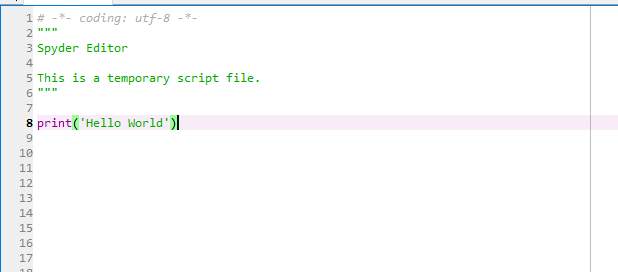
\includegraphics[width=12cm]{section/sp/sp1.png}
	\centering
	\end{figure}
	
	\item run file dan akan terprint "hello World"
	\begin{figure} [h]
	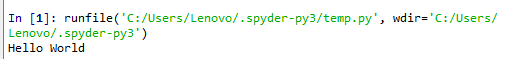
\includegraphics[width=12cm]{section/sp/sp2.png}
	\centering
	\end{figure}
	
	
	
	
\end{enumerate}

\chapter*{Variabel Spyder}

\begin{enumerate}
   

\item buka spyder dan ketikan kode seperti berikut
	\begin{figure} [h]
	
\includegraphics[width=10cm]{section/sp/sp5.png}
	\centering
	\end{figure}
	
	
\item pada kode berikut "jefri" merupakan value dan "nama" merupakan variabel
	\begin{figure} [h]
	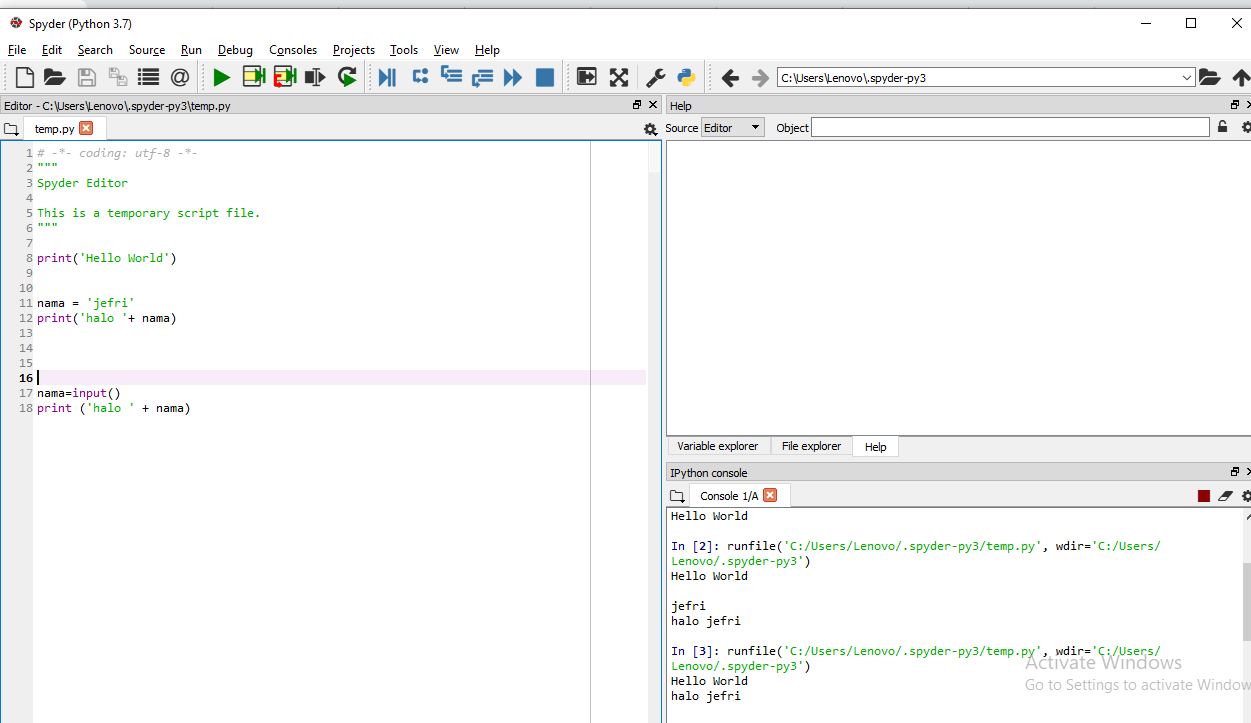
\includegraphics[width=12cm]{section/sp/sp6.png}
	\centering
	\end{figure}
	
 \item maka akan tercetak 
 \begin{figure} [h]
	
\includegraphics[width=6cm]{section/sp/sp7.png}
	\centering
	\end{figure}
 
	
	\end{enumerate}
\chapter*{IDENTASI}

\section*{Penjelasan, membaca error dan menangani Identasi}

\par
Identasi merupakan salah satu bagian paragraf yang menjorok kedalam pada baris didalam paragraf, tidak menggunakan curly brackets "{}" untuk membedakan bagian program digunakan identasi. untuk mengetahui jenis errornya dapat diketahui melalui IndentitionError: expected an idented block. untuk menghindari error ini bisa menggunakan fungsi if memerlukan identasi untuk membedakannya.

\begin{figure} [h]
	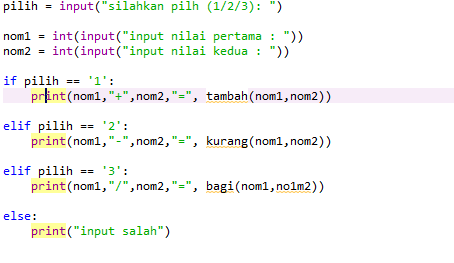
\includegraphics[width=12cm]{section/spy/li.png}
	\centering
	\end{figure}
	
	
	

\chapter*{Cara Membaca Eror }

\begin{enumerate}
	\item Jika terdampat tanda seru atau warning di tab angka itu menandakan terjadi eror pada script, di gambar terdapat pada baris ke 9 
	\begin{figure} [h]
	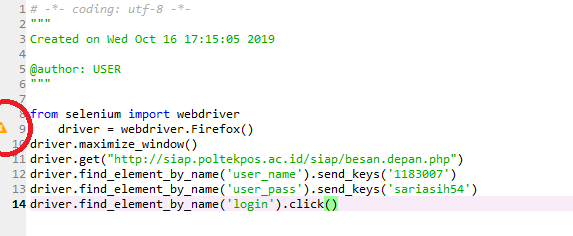
\includegraphics[width=5cm]{identasi/1.png}
	\centering
	\end{figure}
	
	\end{enumerate}
\chapter{Fungsi dan Kelas}
\section{Fungsi}
\subsection{Fungsi}
\par 
Fungsi merupakan suatu blok kode yang berfungsi untuk menampung suatu bari program yang nantinya dapat dieksekusi dengan cara memanggil fungsi tersebut.

\subsection{Parameter}
\par
Parameter adalah sebuah variabel yang dapat menampung suatu nilai yang nantinya dijalan kan pada sebuah fungsi, contohnya.

\begin{lstlisting}[language=Python]

def npm(npm):
	print("hai")
	
\end{lstlisting}

\subsection{Mengembalikan Nilai(\textit{Return}}
\par
Return merupakan sebuah fungsi yang digunakan untuk menampilkan output dari fungsi yang sebelumnya telah dibuat

\begin{lstlisting}[language=Python]
def keliling(kotak):
	keliling = p * l
	return keliling 
\end{lstlisting}

\section{Package}
\subsection{Package}
Package adalah sebuah wadah untuk menyimpan sekumpulan file-file modul.
Cara memanggil sebuah package adalah sebagai berikut

\begin{lstlisting}[language=Python]
form mahasiswa input npm
\end{lstlisting}

\section{Class}
\subsection{Class}
Class merupakan sebuah prototipe/blueprint dari sebuah objek. contohnya class ini akan diberi nama \textbf{satu.py}

\begin{lstlisting}[language=Python]
class Mahasiswa:
	def __init__(self,npm):
		self.npm = npm
	def mhs(self,npm):
		print(npm)
\end{lstlisting}


\subsection{Objek}
Objek merupakan hasil yang telah terdefinisikan dari sebuah class.

\begin{lstlisting}[language=Python]
import satu

test=satu.npm(npm)
\end{lstlisting}

\subsection{Atribut}
Atribut merupakan variabel yang dimiliki suatu class

\begin{lstlisting}[language=Python]
class Mahasiswa:
	def __init__(self,npm):
		self.npm = npm
\end{lstlisting}

\subsection{Method}
Method merupakan kumpulan fungsi-fungsi pada sebuah class

\begin{lstlisting}[language=Python]
class Mahasiswa:
	def __init__(self,npm):
		self.npm = npm
	def mhs(self,npm):
		print(npm)
\end{lstlisting}


\begin{lstlisting}[language=Python]
import satu

test=satu.npm(npm)
\end{lstlisting}

\section{Package}
\subsection{Penggunaan Package}
Buat suatu library terlebih dahulu

\begin{lstlisting}[language=Python]
class Mahasiswa:
	def __init__(self,npm):
		self.npm = npm
	def mhs(self,npm):
		print(npm)
\end{lstlisting}

Import library yang tadi sudah dibuat, dan panggil fungsi yang dibutuhkan
\begin{lstlisting}[language=Python]
import satu

test=satu.npm(npm)
\end{lstlisting}

\section{Import}
\subsection{from kalkulator import penambahan}
\begin{lstlisting}[language=Python]
from kalkulator import penambahan
\end{lstlisting}

Kode tersebut memiliki arti memanggil package kalkulator dan mengimport fungsi penambahan. Contoh code lainnya adalah sebagai berikut.
\begin{lstlisting}[language=Python]
from mahasiswa import npm
\end{lstlisting}

\section{Library}
\subsection{Pemanggilan library dalam folder}
Untuk memanggil sebuah library, pertama kita harus memanggil foldernya terlebih dahulu baru memanggil library yang diiinginkan.
\begin{lstlisting}[language=Python]
from mahasiswa import npm
\end{lstlisting}

\subsection{Pemanggilan class dalam folder}
Untuk memanggil sebuah class, pertama kita harus memanggil foldernya terlebih dahulu baru memanggil library yang diiinginkan.

\end{document}

